\documentclass[usenames,dvipsnames,notes]{beamer}
\usepackage{ifthen}
\usepackage{xcolor}
\usepackage{pgfplots}
\usepackage{amsmath}
\usepackage{centernot}
\usepackage{pifont}
\usepackage{tabularx}
\usepackage{makecell}
\usepackage{cuted}
\usepackage{booktabs}
\usepackage{array}
\usepackage{setspace}
\usepackage{CJKutf8}
\usepackage{textcomp}


%\usepackage{pgfpages}
%\setbeameroption{show notes on second screen}

\pgfplotsset{compat=1.17,
    every axis/.append style={
            font=\large,
            line width=1pt,
            tick style={line width=0.8pt}}}

\input ../beamer-style
\input ../std-macros
\input ../macros

\AtBeginSection[]
{
    \begin{frame}
        \frametitle{Table of Contents}
        \tableofcontents[currentsection]
    \end{frame}
}



\title[CSCI-GA.2590]{Machine Learning Basics}
\author[He He]{He He
}
\institute[NYU]{New York University}
\date{\today}

\begin{document}

\begin{frame}
\titlepage
\end{frame}

\section{Generalization}

\begin{frame}
    {Rules vs data}
    Example: spam filter
    \begin{itemize}
        \itemsep1em
        \item Rules
            \begin{itemize}
                \item[] Contains ``Viagra''
                \item[] Contains ``Rolex''
                \item[] Subject line is all caps
                \item[] ... 
            \end{itemize}
        \item Learning from data
            \vspace{5em}
    \end{itemize}
\end{frame}

\begin{frame}
    {Keys to success}
    \begin{itemize}
        \itemsep1em
        \item Availability of large amounts of (annotated) data
            \begin{itemize}
                \item[] Scraping, crowdsourcing, expert annotation
            \end{itemize}
        \item Generalize to unseen samples
            \begin{itemize}
                \item[] \alert{Unknown} data generating distribution: $\sD$ over $\sX\times\sY$
                \vspace{5em}
            \end{itemize}
    \end{itemize}
\end{frame}

\begin{frame}
    {Empirical risk minimization (ERM)}
    Minimize the average loss on the training set over $\sH$
    \vspace{10em}
\end{frame}

\begin{frame}
    {Error decomposition}
\end{frame}

\begin{frame}
    {Overfitting vs underfitting}
    Trade-off between complexity of $\sH$ (approximiation error) and estimation error

    \vspace{10em}
    \emph{Question for us}: how to choose a good $\sH$ for certain domains
\end{frame}

\section{Optimization}

\begin{frame}
    {Overall picture}
    \begin{enumerate}
        \itemsep2em
        \item Obtain training data $D_{\text{train}}=\pc{(x^{(i)}, y^{(i)})}_{i=1}^n$.
        \item Choose a loss function $L$ and a hypothesis class $\sH$.
        \item Learn a predictor by minimizing the empirical risk.
    \end{enumerate}
\end{frame}

\begin{frame}
    {Gradient descent}
    \begin{itemize}
        \item $w \leftarrow w - \eta\nabla_w F(w)$
        \item Converge to a local minimum (also global minimum if $F(w)$ is \textbf{convex}) with carefully chosen step sizes
    \end{itemize}
    \vspace{10em}
\end{frame}

\begin{frame}
    {Convex optimization (unconstrained)}
    \begin{itemize}
        \item A function $f\colon \BR^d \rightarrow \BR$ is convex if for all $x,y \in \BR^d$ and $\theta \in [0,1]$ we have
            $$
            f(\theta x + (1-\theta)y) \le \theta f(x) + (1-\theta) f(y)  \;.
            $$
        \item $f$ is concave if $-f$ is convex.\\
        \vspace{6em}
        \item Locally optimal points are also globally optimal.
        \item For unconstrained problems, $x$ is optimal iff $\nabla f(x) = 0$.
    \end{itemize}
\end{frame}

\begin{frame}
    {Stochastic gradient descent}
    \begin{itemize}
        \item \textbf{Gradient descent (GD)}
            $$
            w \leftarrow w - \eta\nabla_w \underbrace{\sum_{i=1}^n L(x^{(i)}, y^{(i)}, f_w)}_{\text{training loss}}
            $$
        \item \textbf{Stochastic gradient descent (SGD)}\\
            \begin{align*}
                \text{For each } &(x, y) \in D_{\text{train}}:\\
                &w \leftarrow w - \eta\nabla_w \underbrace{L(x, y, f_w)}_{\text{example loss}}
            \end{align*}
    \end{itemize}
\end{frame}

\begin{frame}
    {GD vs SGD}
    \begin{figure}
        \caption{Minimize $1.25(x + 6)^2 + (y - 8)^2$}
        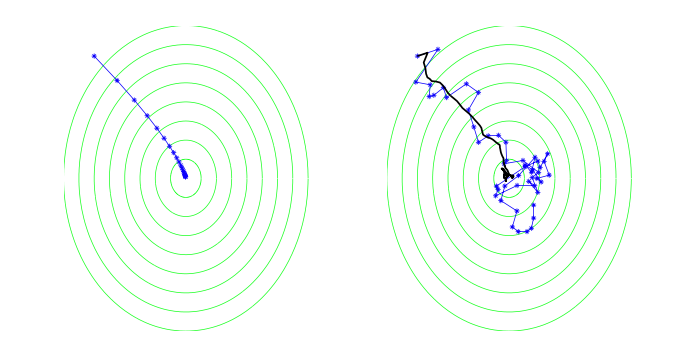
\includegraphics[height=5cm]{figures/gd-vs-sgd}
    \end{figure}
    (\small{Figure from ``Understanding Machine Learning: From Theory to Algorithms''.})
\end{frame}

\begin{frame}
    {Stochastic gradient descent}
    \begin{itemize}
        \itemsep1em
        \item Each update is efficient in both time and space
        \item Can be slow to converge 
        \item Popular in large-scale ML, including non-convex problems
        \item In practice, 
            \begin{itemize}
                \item[] Randomly sample examples.
                \item[] Fixed or diminishing step sizes, e.g. $1/t$, $1/\sqrt{t}$.
                \item[] Stop when objective does not improve.
            \end{itemize}
    \end{itemize}
\end{frame}

\section{Loss functions}

\begin{frame}
    {Zero-one loss}
    \begin{itemize}
        \item Settings
            \begin{itemize}
                \item[] Binary classification: $y\in\pc{+1, -1}$.
                \item[] Scorer $f_w\colon \sX \rightarrow \bR$ parametrized by $w \in \bR^d$.
                \item[] Output prediction: $\text{sign}(f_w(x))$.
            \end{itemize}
        \item Zero-one (0-1) loss
            $$
            L(x, y, f_w) = \1\pb{yf_w(x) \le 0}
            $$
    \end{itemize}
    \begin{figure}
        \includegraphics[height=4cm]{figures/loss}
    \end{figure}
\end{frame}

\begin{frame}
    {Hinge loss}
    $$
    L(x,y,f_w) = \max(1-yf_w(x), 0)
    $$
    \begin{figure}
        \includegraphics[height=4cm]{figures/loss}
    \end{figure}
    Subgradient:\\
    \vspace{4em}
\end{frame}

\begin{frame}
    {Logistic loss}
    $$
    L(x,y,f_w) = \log(1+e^{-yf_w(x)})
    $$
    \begin{figure}
        \includegraphics[height=4cm]{figures/loss}
    \end{figure}
\end{frame}

\begin{frame}
    {Summary}
    \begin{itemize}
        \itemsep2em
        \item Bias-complexity trade-off: choose hypothesis class based on prior knowledge
        \item Learning algorithm: empirical risk minimization
        \item Optimization: stochastic gradient descent
    \end{itemize}
\end{frame}

\end{document}
